\section{Python}
\begin{frame}{Python}
  \begin{center}
    
\includegraphics[width=140px]{img/python.png} \\
    \color{TUgreen}\textbf{\href{http://python.org}{www.python.org}}
  \end{center}
  \begin{quote}
    \begin{spacing}{1.0}
      Python is a programming language that lets you work more quickly and integrate your systems more effectively.
      You can learn to use Python and see almost immediate gains in productivity and lower maintenance costs.
    \end{spacing}
  \end{quote}
\end{frame}

\begin{frame}{Python ist...}
  \begin{itemize}
    \item […] eine Programmiersprache.
    \item […] einfach!
    \item […] sehr mächtig.
    \item […] universell einsetzbar.
  \end{itemize}
  \begin{center}
    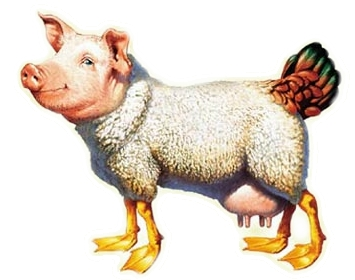
\includegraphics[width=120px]{img/eierlegendewollmilchsau.jpg}\\
    \tiny\texttt{\href{http://xn--sptzlemitsoss-cfb.de/wp-content/uploads/2012/07/eierlegendewollmilchsau.jpg}{http://xn--sptzlemitsoss-cfb.de/wp-content/uploads/2012/07/eierlegendewollmilchsau.jpg}}\normalsize
  \end{center}
\end{frame}

\begin{frame}[fragile]{Ein kleines Beispiel}
  \vspace{-1em}
  \begin{columns}
    \begin{column}{0.5\textwidth}
      \begin{exampleblock}{C++}
        \begin{minted}[fontsize=\footnotesize]{c++}
#include <iostream>
using namespace std;
int main(int argc, char *argv[])
{
    cout << "Hello, World!" << endl;
    return 0;
}
        \end{minted}
      \end{exampleblock}
    \end{column}
    \begin{column}{0.5\textwidth}
      \begin{exampleblock}{Python}
        \begin{minted}[fontsize=\footnotesize]{python}
print("Hello, World!")
        \end{minted}
      \end{exampleblock}
    \end{column}
  \end{columns}
\end{frame}

\begin{frame}{Python}
  \tableofcontents[sectionstyle=show/hide,
                   subsectionstyle=show/show/hide,
                   subsubsectionstyle=show/show/show]
\end{frame}

\subsection{IPython}
\begin{frame}{IPython}
  \begin{center}
    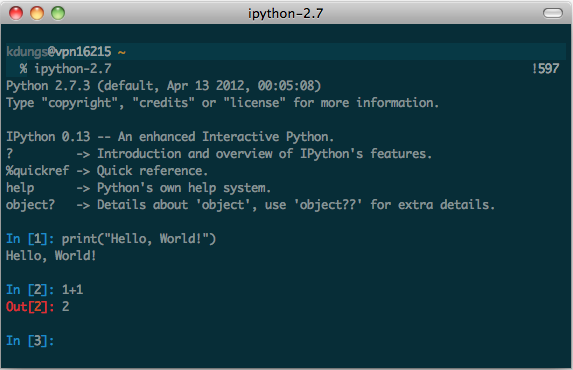
\includegraphics[width=300px]{img/ipython.png}
  \end{center}
\end{frame}

\subsection{Syntax}
\begin{frame}{Syntax}
  \begin{block}{Blöcke}
    \begin{itemize}
      \item Durch Einrückung!
      \item 4 Leerzeichen (/1 Tab)
    \end{itemize}
  \end{block}
  \begin{block}{Semikolons}
  \begin{itemize}
    \item Gibt es prinzipiell
    \item Sind am Zeilenende aber nicht notwendig
  \end{itemize}
  \end{block}
\end{frame}

\begin{frame}[fragile]{Variablen}
  \begin{itemize}
    \item Dynamische Typisierung
    \item Keine explizite Deklaration 
  \end{itemize}
  \begin{spacing}{1.0}
    \begin{exampleblock}{Beispiel}
      \begin{minted}{python}
In [1]: a = 1

In [2]: b = 2

In [3]: name = "Kääähbiiin"

In [4]: a, b, name
Out[4]: (1, 2, 'Kääähbiiin')
      \end{minted}
    \end{exampleblock}
  \end{spacing}  
\end{frame}

\begin{frame}{Datenstrukturen}
  \begin{itemize}
    \item bool (\texttt{True}, \texttt{False})
    \item int, float, long, complex
    \item string (\texttt{'foo'}, \texttt{"bar"})
    \item Iteratoren, Generatoren, Sequenzen, …
  \end{itemize}
\end{frame}

\begin{frame}[fragile]{Datenstrukturen}
  \begin{block}{Praktische Typen}
    \begin{itemize}
      \item[\texttt{()}] Tupel
      \item[\texttt{[]}] Liste
      \item[\texttt{\{\}}] Dictionary 
    \end{itemize}
  \end{block}
  \vspace{.5em}
  \begin{spacing}{1.0}
    \begin{exampleblock}{Zum Beispiel}
      \begin{minted}{python}
In [9]: cities = ['Dortmund', 'Hamburg', 'Berlin']

In [10]: cities[0]
Out[10]: 'Dortmund'
      \end{minted}
    \end{exampleblock}
  \end{spacing}
\end{frame}

\begin{frame}[fragile]{Mehr Beispiele}
  \begin{minted}{python}
In [1]: teams = {
   ...:         'BVB': "BV Borussia Dortmund 09",
   ...:         'S04': "FC Schalke 04",
   ...:         'FCB': "FC Bayern München"
   ...: }

In [2]: teams['BVB']
Out[2]: 'BV Borussia Dortmund 09'
  \end{minted}
\end{frame}

\begin{frame}[fragile]{Operatoren}
  \begin{spacing}{1.0}
    \begin{block}{Arithmetische Operatoren}
      \begin{minted}{python}
+, -, *, /, %, **, //
      \end{minted}
    \end{block}
    \begin{block}{Zuweisungsoperatoren}
      \begin{minted}{python}
=, +=, -=, *=, /=, %=, **=, //=
      \end{minted}
    \end{block}
    \begin{block}{Vergleichsoperatoren}
      \begin{minted}{python}
==, !=, <, <=, >, >=
      \end{minted}
    \end{block}
  \end{spacing}
\end{frame}

\begin{frame}[fragile]{Operatoren}
  \begin{spacing}{1.0}
    \begin{block}{Logische Operatoren}
      \begin{minted}{python}
and, or, not
      \end{minted}
    \end{block}
    \begin{block}{Identitätsoperatoren}
      \begin{minted}{python}
is, is not
      \end{minted}
    \end{block}
    \begin{block}{Operatoren für Sequenzen}
      \begin{minted}{python}
in, not in
      \end{minted}
    \end{block}
  \end{spacing}
\end{frame}

\begin{frame}[fragile]{Kontrollstrukturen}
  \begin{spacing}{1.0}
    \begin{block}{if}
      \begin{minted}{python}
if condition:
    # do something
elif other_condition:
    # or do something else
else:
    # or something else
      \end{minted}
    \end{block}
    \begin{block}{case}
      gibt es \emph{nicht}!
    \end{block}
  \end{spacing}
\end{frame}

\begin{frame}[fragile]{Schleifen}
  \begin{block}{while}
    \begin{minted}{python}
while condition:
    # do something
    \end{minted}
  \end{block}
  \begin{block}{for}
  \begin{itemize}
   \item \texttt{for … in}
   \item agiert immer auf \emph{Sequenzen}!
  \end{itemize}
  \end{block}
\end{frame}

\begin{frame}[fragile]{for - Beispiele}
\vspace{-1em}
\begin{spacing}{1.0}
\begin{columns}
    \begin{column}{0.4\paperwidth}
      \begin{exampleblock}{Listen}
        \begin{minted}{python}
for city in cities:
    print(city)
    
Dortmund
Hamburg
Berlin
        \end{minted}
      \end{exampleblock}
    \end{column}
    \begin{column}{.4\paperwidth}
      \begin{exampleblock}{Range}
        \begin{minted}{python}
for i in range(0, 10):
    print(i)
    
0
1
2
3
…
        \end{minted}
      \end{exampleblock}
    \end{column}
  \end{columns}
\end{spacing}
\end{frame}

\begin{frame}[fragile]{Funktionen}
  \begin{block}{Aufruf}
    \begin{itemize}
      \item \texttt{print(something)}
      \item \texttt{funktionsname(*args, **kwargs)}
    \end{itemize}
  \end{block}
  \begin{block}{Definition}
    \begin{minted}{python}
def funktionsname(param1, param2=defaultwert, ...):
  # do something
    \end{minted}
  \end{block}
\end{frame}

\begin{frame}[fragile]{Module}
  \begin{itemize}
    \item \texttt{import modulname}
    \item \texttt{import modulname as alias}
    \item \texttt{from modulname import teil}
    \item \texttt{from modulname import *}
  \end{itemize}
  \begin{exampleblock}{Zum Beispiel}
    \begin{minted}{python}
import numpy as np
a = np.array([1, 2, 3])
    \end{minted}
  \end{exampleblock}
\end{frame}

\begin{frame}[fragile]{Und ohne IPython?}
  \begin{itemize}
    \item Dateiendung \texttt{.py}
    \item Aufruf per \texttt{python3 dateiname.py}
    \item \texttt{print()}-Funktion 
  \end{itemize}
\end{frame}

\subsection{Bibliotheken}
\subsubsection{NumPy}
\begin{frame}{NumPy}
  \begin{itemize}
    \item $n$-dimensionale Arrays
    \item Funktionen, die auf denen arbeiten
    \item Operatoren wirken elementweise
    \item wird meist mit \texttt{np} abgekürzt
  \end{itemize}

  Konstanten:
  \begin{itemize}
    \item \texttt{pi}
    \item \texttt{e}
  \end{itemize}
\end{frame}

\begin{frame}{Arrays erstellen}
  \begin{itemize}
    \item \texttt{array}: konvertiert irgendwas (Liste, Tupel, …) zu einem Array
    \item \texttt{linspace(start, end, number)}: \texttt{number} Zahlen zwischen \texttt{start} und \texttt{end} in gleichem Abstand
    \item \texttt{arange(start, end, step)}: Zahlen zwischen \texttt{start} und \texttt{end} mit dem Abstand \texttt{step}
    \item \texttt{zeros(shape)}: Array aus Nullen der Größe \texttt{shape}
    \item \texttt{ones(shape)}: Array aus Einsen der Größe \texttt{shape}
  \end{itemize}
\end{frame}

\begin{frame}{Elementweise Funktionen}
  Beispiele:
  \begin{itemize}
    \item \texttt{sqrt}
    \item \texttt{exp}, \texttt{log}
    \item \texttt{sin}
    \item \texttt{deg2rad}, \texttt{rad2deg}
  \end{itemize}
\end{frame}

\begin{frame}{Reduzierende Funktionen}
  Beispiele:
  \begin{itemize}
    \item \texttt{sum}
    \item \texttt{mean}
    \item \texttt{max}, \texttt{min}
    \item \texttt{ediff1d}
  \end{itemize}
\end{frame}

\begin{frame}{It/Output}
  \begin{itemize}
    \item \texttt{loadtxt(file [, unpack=True])}: Lädt eine Datei in ein Array.
      \texttt{unpack=True} transponiert das Array
    \item \texttt{savetxt(file, array)}: Speichert ein Array in eine Datei
  \end{itemize}
\end{frame}

\subsubsection{SciPy}
\begin{frame}{SciPy}
\end{frame}

\begin{frame}{Nützliche Funktionen}
  \begin{itemize}
    \item \texttt{optimize.curve\_fit}: fittet nichtlineare Funktionen
    \item \texttt{stats.sem}: gibt den Fehler des Mittelwerts
    \item \texttt{constants.C2K}: konvertiert Celsius in Kelvin
    \item \texttt{constants.K2C}: konvertiert Kelvin in Celsius
  \end{itemize}
\end{frame}

\begin{frame}{Konstanten}
  \begin{itemize}
    \item \texttt{scipy.constants.physical\_constants}: enthält diverse physikalische Konstanten, ihre Fehler und Einheiten (aus CODATA)
  \end{itemize}
\end{frame}

\subsubsection{matplotlib}
\begin{frame}{matplotlib}
\end{frame}
\subsubsection{PyLab}
\begin{frame}{PyLab}
\end{frame}
